\chapter{Marco teórico}
\label{capitulo1}
\lhead{Capítulo 2. \emph{Marco teórico}}


En el siguiente cap\'itulo se describir\'an algunos conceptos importantes para comprender la implementaci\'on del sistema del que se hablar\'a en el presente trabajo. Dichos conceptos son: \textit{IDS, el protocolo HTTP, URI , autom\'atas de estados finitos, autom\'atas probabilisticos, modelo de Markov,SSM y Bro}.

En l\'ineas generales, el trabajo, tiene como prop\'osito explicar la implementaci\'on de un \textit{IDS} híbrido que haga uso del sistema \textit{SSM} a traves del lenguaje de scripting de la herramienta \textit{BRO}.

El sistema analizar\'a los \textit{URI} de las peticiones tipo GET del protocolo \textit{HTTP}, haciendo uso de la t\'ecnica \textit{SSM}. Esta t\'ecnica, a su vez hace uso \textit{automatas de estados finitos probabilisticos} y del \textit{modelo de Markov} para determinar si ciertas peticiones realizadas a un servidor HTTP son posibles ataques o no.
% De qué va a tratar el capítulo
% El capítulo 1 suele ser el marco teórico.

\section{Detector de intrusiones (IDS)}
Un detector de intrusiones o IDS por sus siglas en ingl\'es (intrusion-detection system) a manera general es un sistema que se encarga de procesar la informaci\'on entrante de un sistema a proteger.

La intenci\'on de tomar la informaci\'on entrante es la de realizar un diagnostico de seguridad para as\'i descubrir los posibles ataques, brechas de seguridad o vulnerabilidades que pueden existir en el sistema que se quiere proteger.

Existen diversos tipos de IDS. Pero los mas comunes son los IDS basados en firmas, los IDS basados en comportamiento y los IDS h\'ibridos que son una mezcla entre un IDS basado en firma y un IDS basado en comportamiento.

Los IDS basados en firmas, utilizan una base de datos que contiene una lista de posibles ataques que pueden ser perpetuados y las vulnerabilidades del sistema. Entonces, el IDS cuando esta filtrando la informaci\'on que va a entrar al sistema compara esa o parte de la informac\'on con la base de datos de ataques, si dentro de la informaci\'on entrante existe una firma que se encuentra en la base de datos entonces se activar\'a una alarma para indicar que un ataque esta siendo perpetuado. De otro modo, la informaci\'on entrante ser\'a  catalogada como aceptable.

La eficacia de los detectores de intrusiones basados en firmas es muy buena, sin embargo, su buen funcionamiento depende completamente de la constante actualización de la base de datos de ataques.


Por otra parte, est\'an los IDS basados en comportamiento que detectan los ataque de manera diferente. En este tipo de IDS los ataques son detectados a partir de la observaci\'on del comportamientos, bien sea del sistema o de los usuarios. 

El modo de funcionamiento de un IDS basado en comportamiento se basa en, recolectar la informaci\'on entrante del sistema a proteger y comparar dicha informaci\'on con un modelo de normalidad del sistema que ha sido previamente construido. El modelo de normalidad se construye a partir de comportamientos previamente observado en el sistema y que son catalogados como "normales". Si existe una incongruencia muy grande entre la informaci\'on entrante y el modelo de normalidad, entonces se generar\'a una alarma.

No obstante, uno de los problemas que posee este tipo de detector de instrusiones es la alta tasa de falsos positivos que puede llegar a tener. Esto se debe a que es casi imposible que un modelo posea todos los comportamientos normales de un sistema en su totalidad, lo cual provocar\'ia que informac\'on que est\'a libre de ataques sea catalogada como una amenaza. Tambi\'en esta el hecho de que es muy posible que con el pasar del tiempo, el comportamiento del sistema a proteger vaya cambiando lo cual implicar\'ia que si no se hace una constante revis\'on del y reentrenamiento modelo de normalidad el mismo quedar\'a obsoleto y la informaci\'on entrante ser\'a mal catalogada por el IDS. El problema de realizar entrenamientos constantes para actualizar un modelo de normalidad es que, a pesar de que el modelo contendr\'a una informaci\'on acertada acerca del comoportamiento del sistema se crear\'an brechas de tiempo en donde el sistema ser\'a muy vulnerable a ataques ya que en lugar de estar funcionando el modulo para detectar ataques estar\'a funcionando el modulo para entrenar el modelo de normalidad. Por lo tanto, si un ataque es perpetuado durante ese periodo de tiempo el mismo quedar\'a grabado en el modelo de normalidad como un comportamiento normal del sistema.

As\'i mismo tambi\'en existen los IDS h\'ibridos cuyo funcionamiento mezcla el funcionamiendo de los detectores de instrusiones basados en firma y los basados en comportamiento. En pocas palabras, los IDS h\'ibirdos suelen contar con una base de datos de ataques y tambi\'en con un modelo de normalidad.

El IDS implementado es de t\'ipo h\'ibrido ya que por una parte, se revisan las firmas (en este caso los URI) de la informaci\'on entrante, y si estas no muestran ninguna incongruencia, dicha informaci\'on pasar\'a a ser contrastada con el modelo de normalidad. S\i la misma es muy diferente a dicho modelo, entonces se emitir\'a una alarma.

\section{Protocolo HTTP}

Definici\'on:

Hypertext Transfer Protocol (HTTP) seg\'un el RFC 7230 es un protocolo cliente/servidor que funciona a nivel de capa de aplicaci\'on y cuya funci\'on es transferir hipertexto a traves de la red.\\

 Este protocolo es considerado una de las bases fundamentales dentro de la comunicaci\'on de datos en el Internet.\\
 
 El cliente de un protocolo HTTP es un programa que se encarga de crear una conexi\'on con el servidor y enviar las diferentes peticiones de recursos al mismo. Por su parte, el servidor HTTP se encargar\'a de aceptar dicha conex\'on y responder a las peticiones hechas por el cliente.\\
 
Los recursos de este protocolo son identificados por un Uniform Resource Identifier (URI).\\

Por otra parte, este protocolo posee diferentes metodos para solicitar las peticiones de recursos. Estos son, el m\'etodo GET, HEAD, POST, PUT, DELETE, CONNECT, OPTIONS, TRACE. \\

Los m\'etodos GET, HEAD y POST son los mas utilizados en las comunicaciones del protocolo HTTP. El m\'etodo GET, consiste en solicitar de un cierto recurso al programa servidor HTTP. Por su parte,el m\'etodo POST se utiliza para informar al destinatario que procese la informaci\'on que viene incluida en la solicitud realizada y el m\'etodo HEAD, funciona de manera identica al m\'etodo GET con la \'unica diferencia de que la solicitud solo ser\'a respondida con la cabecera del recurso excluyendo el cuerpo del mismo.\\

    
\section{URI} \label{URIsection}

Seg\'un el RFC 3986 un URI (Uniform Resource Identifier) es una serie de caracteres que identifican un recurso en la red. Este tiene una sintaxis especifica que esta conformada por diferentes segmentos de caracteres para el esquema, la autoridad, la ruta, el query y el fragment.

A continuaci\'on se describen de manera breve cada uno de los componentes que pueden conformar un URI.

\begin{itemize}

\item Esquema:

El esquema identifica el protocolo que va a ser utilizado. En el caso del presente trabajo, los URIs utilizaran unicamente el protocolo http o https.


\item Authority:

Este componente del URI posee informaci\'on del usuario que pueden ser nombres de usuarios y contraseñas (campo opcional), el host y el puerto correspondiente (campo opcional).

El host de un URI viene representado bien sea por un IPv4 o un nombre de dominio, seguido de un n\'umero de puerto (opcional) que identifican la m\'aquina en donde est\'an los recursos a solicitar.
   
\item Path:
La ruta de un URI son un conjunto de segmentos organizados de manera jerarquica y separados por slashes que contienen informaci\'on sobre la ubicaci\'on de los recursos a solicitar.

\item Query:

El query de un URI es un segmento de informaci\'on no jerarquizada, cuyo simb\'olo de inicio es el signo de interrogaci\'on (?). Por lo general, el query est\'a conformado por una dupla "atributo=valor" que junto con la ruta ayudan a identificar el recurso que se desea solicitar. No obstante, a diferencia de la ruta, la informaci\'on aqu\'i contenida debe ser procesada por el servidor al que se le esta solicitando el recurso. 

Por otra parte, el atributo, representa el nombre de una variable y el valor vendria siendo el valor que contendr\'a dicha variable.

\item Fragment:

En un URI, el fragment corresponde a la direcci\'on de un segundo recurso dentro del primer recurso identificado por la ruta y el query. Esta cadena de caracteres esta precedida por el simbolo de un numeral (\#).

\end{itemize}

En un URI, tanto el esquema como la ruta son segmentos que deben existir de manera obligatoria. Si la ruta es un caracter vac\'io, se asumir\'a que la misma es "/". El resto de los segmentos son opcionales.


\begin{figure}
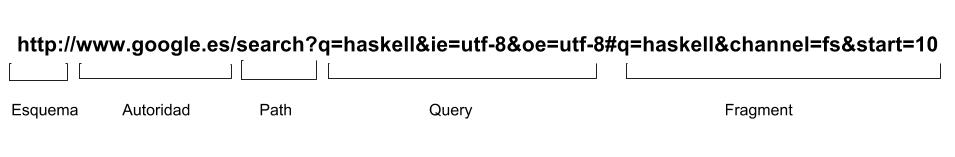
\includegraphics[width=\linewidth]{./URI.jpg}
\caption{URI.}
\label{fig:URI}
\end{figure}

En la figura \ref{fig:URI}, se muestra, en un ejemplo los componentes que forman un URI.


\section{Autom\'atas de estados finitos}

Los automatas son modelos muy importante dentro de las ciencias de la computaci\'on. Su presencia est\'a  en diversos ambitos de esta ciencia. Desde programas para hacer la verificaci\'on de protocolos de comunicaci\'on, analizadores sint\'acticos de compiladores,programas que realizan la verificaci\'on del comportamiento de circuitos digitales o el escaneo de largos bloques de texto.

Antes que nada es preciso recalcar que existen dos tipos de automatas de estados finitos: los automatas deterministas y los no deterministas.

Los automatas deterministas son aquellos que para cada input solo existe un estado del automata al cual se puede transitar.

Formalmente, un automata determinista, A, se puede representar de la siguiente manera:

A = (Q,$\Sigma,\delta,q_{0},F$)\\

Donde:

\begin{itemize}

\item Q : Es un conjunto de estados.
\item $\Sigma$ : Es un conjunto de simbolos, tambien llamado alfabeto.

\item $\delta$ : Es una funci\'on de transici\'on que toma como argumento un estado y un simbolo y retorna un estado, es decir, $\delta$ : Q x $\Sigma$ $\rightarrow Q.$
Si el automata es representado como un grafo, entonces esta funci\'on de trasnsici\'on vendria representada por el arcco que une dos nodos junto al simbolo del mismo.

\item $q_{0}$: Es el estado inicial del automata.

\item F : Es un conjunto de estados finales.

\end{itemize}

A continuaci\'on se presentar\'a un ejemplo de un automata.

A = (\{X,Z\},\{a,b\},\{$\delta(X,a)=Z,\delta(Y,b)=X$\},\{X\},\{Z\})

 El mismo ser\'a representado a traves de un grafo, en donde los nodos representar\'an los estados del automata, y los arcos junto a sus simbolos representaran las funciones de transici\'on en la figura \ref{fig:automata}.

\begin{figure}
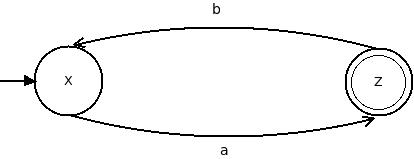
\includegraphics[width=\linewidth]{./automata.jpeg}
\caption{Automata determinista.}
\label{fig:automata}
\end{figure}

Por otra parte, los automatas no deterministas, a diferencia de los automatas deterministas pueden tener un conjunto de estado en el automata al cual se puede transitar para cada input, es decir, la funci\'on de transici\'on de un automata no determinista en lugar de devolver solo un estado dado un simbolo y un estado puede devolver un conjunto de estados.

La representaci\'on de los mismos es analoga a la de los automatas deterministas con la diferencia que $\delta$ estar\'ia definida como una funci\'on de transici\'on de la siguiente forma $\delta$ : Q x $\Sigma$ $\rightarrow \{Q\}.$

\section{Modelo de Markov}

Un modelo de Markov los eventos futuros dependen de los eventos anteriores, es decir, son procesos con memoria.

Un modelo de Markov discreto, $\lambda$, se define de la siguiente forma:

$\lambda$ = (Q,$\Theta$,A,B,$\Pi$)\\

Donde: 

\begin{itemize}
\item Q = {} es el conjunto de N estados del modelo.
\item $\Theta$ es el vocabulario del modelo, es decir, son los posibles s\'imbolos o eventos observables del sistema.
\item A es una matriz NxN de probabilidades de transici\'on entre estados.
A = $[a_{ij}], 1\leq i \leq N  y  1\leq j \leq N.$\\
$a_{ij}$ = P($q_{t}$ = $S_{j}$ | $q_{t-1}$ = $S_{i}$)
\item B es una matriz NxM de probabilidades de generaci\'on u observaciones de los s\'imbolos entre estados.\\
B = $[b_{ik}], 1\leq i \leq N  y  1\leq k \leq M.$\\
$b_{ik}$ = P($O_{t}$ = $v_{k}$ | $q_{t}$ = $S_{i}$)
\item $\Pi$ es el vector de probabilidades del estado inicial.
$\Pi$ = $[\Pi_{i}], 1\leq i \leq N $\\
$\pi_{i}$ = P($q_{1}$ = $S_{i}$)
\end{itemize}

\section{SSM}\label{sec:modeloSSM}

SSM o Structural Stochastic Modeling en ingl\'es es una tecnica desarrollado por Estevez y Tapiador. A grandes rasgos, esta t\'ecnica “se basa en la definición de un autómata de estados finitos estocástico capaz de evaluar la probabilidad de generación de una petición concreta. El autómata permitirá, por tanto, dada una petición, evaluar si dicha petición es legítima (corresponde al modelo) y su probabilidad. En función de la probabilidad y de un umbral se clasificaran las peticiones como normales o anormales” J.E. Díaz-Verdejo, P. García-Teodoro, P. Muñoz, G. Maciá-Fernández, F. De Toro. 2007. Una aproximación basada en Snort para el desarrollo e implantación de IDS híbridos.

Es importante recalcar que esta t\'ecnica adem\'as se basa en la teor\'ia de los modelos de Markov ya que se define un automata de estados finitos y a partir de este se permite evaluar y saber cual es la probabilidad de generaci\'on de una petici\'on dado un modelo previamente construido.

Por otra parte, en el presente trabajo, las peticiones que ser\'as estudiadas por dicha t\'ecnica ser\'an peticiones de tipo GET del protocolo HTTP. En concreto, de las peticiones GET el elemento a estudiar ser\'an los URIs de dichas peticiones. No obstante, el tipo de peticiones se puede extender para que funcione con m\'etodos de tipo POST y HEAD. 

\begin{figure}

  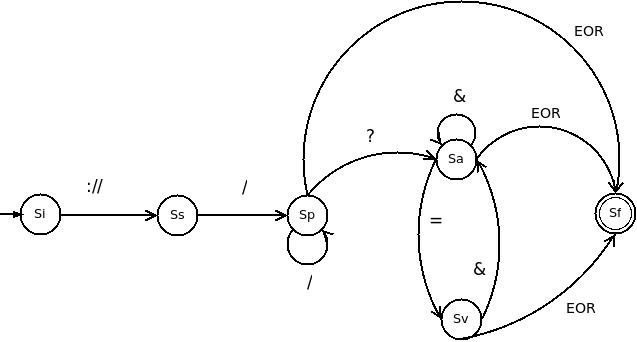
\includegraphics[width=\linewidth]{ssm.jpeg}
  \caption{Automata del modelo SSM}
  \label{fig:ssm}

\end{figure}

Este hecho hace que el automata de SSM deba tomar una cierta topolog\'ia para que de esta forma se puedan reconocer los URIs de cada petici\'on. Dicha topolog\'ia se infiere con ayuda de la sección \ref{URIsection}, en donde se explica tanto la sint\'axis de los URIs como el modo de segmentar los mismos. En la figura \ref{fig:ssm} se muestra la topolog\'ia del automata inferida.

Las transiciones del automata vienen dada por las especificaciones de las sintaxis de los URIs que est\'an descritas en el RFC 3986. Adem\'as, se puede observar en la im\'agen que el n\'umero de estados es casi el mismo que el n\'umero de segmentos de un URI que se presenta en la secci\'on \ref{URIsection} . En el automata, se tiene un estado inicial ($S_{I}$), un estado del host ($S_{S}$), un estado de segmento de ruta ($S_{P}$), un estado atributo ($S_{A}$), un estado valor ($S_{V}$), un estado final ($S_{F}$) y un estado sumidero ($S_{OOS}$) en el que se termina\'ra si el URI no es sint\'acticamente correcto.

Si en una petici\'on del protocolo HTTP viene anexado un URI que no puede ser reconocido por el automata descrito con anterioridad implicar\'a que el URI de dicha petici\'o no est\'a bien construido sintacticamente.

Adem\'as de esto, existir\'a un vocabulario diferente para los estados $S_{S}$, $S_{P}$, $S_{A}$ y $S_{V}$ en donde se encuentren las posibles palabras que puedan aparecer en los mismos.Estos vocabularios son construidos a partir de tomar m\'ultiples peticiones libres de ataques realizadas al servidor. 

Entonces, en pocas palabras lo que hace la t\'ecnica de SSM para detectar intrusiones es verificar la correctitud de la sintaxis del URI de las peticiones enviadas al servidor a traves del automata descrito con anterioridad y al mismo tiempo, se estudia segmento por segmento del URI la probabilidad que tiene cada palabra de aparecer en un estado determinado del automata para as\'i verificar si el URI que viene anexado al la petici\'on es una cadena de caracteres que probabilisticamente corresponde a un petici\'on normal o no.

Por lo tanto, el modelo teorico utilizado por SSM es el siguiente:

\begin{itemize}
\item Q: es el conjunto de estados ($S_{I}$,$S_{S}$,$S_{P}$,$S_{A}$,$S_{V}$,$S_{F}$,$S_{OOS}$).
\item $\theta$: es el conjunto de s\'imbolos observables que se encuentran en el vocabulario de cada estado.
\item A: es la matriz de probabilidad de transiciones entre estados
\item B: es un conjunto de vectores que contiene la probabilidad de las palabras observadas en cada estado. ($B_{I}$,$B_{S}$,$B_{P}$,$B_{A}$,$B_{V}$,$B_{F}$,$B_{OOS}$).
\item $\Pi$: es el vector de probabilidades iniciales, cuyos valores est\'an determinados por la topolog\'ia del modelo. 
\end{itemize}

\section{Bro}

Bro es un software open source cap\'az de analizar a detalle las actividades que ocurren en la red.

Por otra parte, este software incluye un lenguaje de scripting orientado a eventos cuya funci\'on es extender y personalizar las funcionalidades primarias que otorga Bro. 

Este lenguaje de scripting cuenta con una cola de eventos de tipo FIFO y un manejador de eventos que se encarga de servir a los mismos.

Cuenta, adem\'a con un tipo de registro especial que almacena la informaci\'on del estado de las conexiones durante su tiempo de vida.

Por otra parte, dispone de los tipos de datos comunes que encontramos en la mayor\'ia de los lenguajes de programaci\'on como el "int", que representa los n\'umeros enteros de 64 bits, "double" que representa los n\'umeros flotantes de 64 bits, "bool" que representa los booleanos y "count"  que representa los n\'umeros enteros sin signo de 64 bits. Adem\'as de estos tipos de datos el lenguaje de scripting de Bro posee otro tipos de datos  mas especificos para poder trabajar el an\'alisis de redes de manera mas c\'omoda como son el "addr" que es un tipo de datos destinado a las direcciones ip, "port" para los puertos de la capa de transporte, "subnet" para las mascaras de subred, "time" para almacenar datos que representen tiempo, "interval" para representar intervalos de tiempo y "pattern" para las expresiones regulares.

Adem\'as, tine estructura de datos como: conjuntos, tablas, vectores y registros.

As\'i mismo, el lenguaje de scripting de Bro posee un framework que permite manejar de manera c\'omoda y sencilla los logs del sistema y otro para leer de manera eficiente la informaci\'on dentro de los mismos. Con el primero, se puede crear archivos, escribir datos de forma organizada y filtrar informac\'on de los logs. El segundo framework lee la informaci\'on que se encuentra dentro de los logs para luego ser almacenada en tablas o activar cierto evento anteriormente programado.
